% What is a side channel?
A side-channel is a method of extracting information from a program by observing its functionality and environment, rather than through its intended input or output. 
Extracting information from side-channels becomes particularly viable when a program has shared resources with other untrusted entities. 
When an adversary shares resources with the victim's program, it can observe victim's resource usage pattern.
The adversary then can leverage the correlation between resource usage pattern (side-channels) and victims' secrets to breach their privacy. 
A side-channel leak comprises two essential steps: Profiling and Inference.
During profiling, the adversary extracts the correlation between the victim's secrets and their resource usage patterns.
This involves monitoring various resource usage patterns that emerge during the program's execution.
In the inference step, the adversary utilizes the prior knowledge acquired in the first step to infer the victim's secrets based on the observations of resource usage patterns.
One trivial solution to address side-channel leaks is to isolate the program and all its dedicated resources such as CPUs, memory, storage, and network resources at all possible level down to hardware. 
However, this approach often results in inefficient resource utilization, as the resources that the program does not currently use remain idle. 
Moreover, many programs rely on inherently shared resources, such as a common network infrastructure.
Therefore, mitigating side-channels leaks is intrinsically challenging. 

% What are network side channels 
Network applications such as web browsers, email clients, video conferencing software, file-sharing services, and online gaming platforms are exceedingly popular these days.
All these programs utilize a network (\eg Internet) to communicate and exchange data with other devices or systems, while relying on encryption techniques to ensure the privacy of users.
However, the encryption does not conceal packet sizes and timing transmitted by an application, which is correlated with users' sensitive information in many applications.
In a network side-channel attack, by utilizing this correlation, an adversary with control over the underlying network links (e.g., Internet Service Providers) can monitor the traffic pattern and potentially reveal the content of the communication.
Recent advancements in machine learning have significantly empowered the inference step of network side-channel attacks, providing adversaries with enhanced capabilities to effectively map observations to the victim's sensitive information~\cite{schuster2017beautyburst, bhat2019varcnn, hayes2016kfp, sirinam2018df}.

In this section, we first elaborate on the threat model that we consider in {\sys} design. 
We, then, conduct an overview of recent network side-channel attacks, elaborating on both their strengths and weaknesses.
We organize these methods according to their target network applications.
Ultimately, we present our novel TCN-based~\cite{bai2018empirical} network side-channel attack specifically designed to target video services.

\subsection{{\sys} Threat Model}\label{subsec:threat-model}
We assume that the communicating parties are inside separate trusted private networks (\eg each node is behind a VPN gateway node), which an adversary cannot compromise.
We assume that all the application endpoints are non-malicious and do not leak the secrets themselves.
The adversary with control over the underlying network links (e.g., Internet Service Providers) can monitor, manipulate, and record the victim's traffic pattern.
In particular, it can precisely record the traffic shape---the sizes, timing, and direction of packets---on all links in the victim's traffic communication graph.
Furthermore, the adversary can drop, replay, or inject packets into the victim's traffic.
However, it cannot break standard cryptography, cannot compromise the victim's VPN, or cannot impersonate its clients or servers to directly interact with the victim (thus, no covert attacks).
We do not consider threats due to observing the IP addresses of packets.
We also do not consider the threat where a victim accidentally installs a malicious script in the browser, thus enabling an adversary to colocate with the
victim's application and observe its traffic~\cite{schuster2017beautyburst,mehta2022pacer}.
This is a reasonable assumption, since a colocated adversary can exploit many other direct or indirect channels for data leaks that will be far more efficient than {\nsc}s~\cite{kocher2018spectre, yarom2014flushreload, liu2015llcpractical, irazoqui2015ssa, vila2017loophole}.

In this project, we focus on the design of {\sys}'s traffic shaping tunnel
within a middlebox that can be placed in front of the gateway router of an
organization. 
Furthermore, we simulate shaping mechanism of {\sys} and evaluate its privacy and overheads.

{\sys}'s trusted computing base (TCB) includes all components in the organization's private network and the middleboxes.
We assume that the middleboxes do not directly leak application secrets to the adversary.
We assume the cryptographic libraries are side-channel free~\cite{almeida2016verifying}.

{\sys} does not address leaks of one application's sensitive data through the traffic shape of colocated applications transmitting only non-sensitive traffic.
Such leaks may arise, for instance, due to microarchitectural interference among the applications colocated on a host or among their flows if they pass through shared links.
Mitigating such leaks would require physically isolating the
applications and their flows.
For instance, a service serving both privacy-sensitive and privacy-insensitive clients may be partitioned into two instances, with each instance dedicated to serving clients with similar privacy requirements.
For the privacy-sensitive clients, we assume the corresponding service instance agrees to serve the clients according to their privacy requirements. 
Alternatively, end hosts could implement mitigations for various side channels to support colocated applications \cite{mehta2022pacer, page05partitionedcache, shi2011limiting, kim2012stealthmem, varadarajan2014scheduler, braun2015robust}. 
To mitigate leaks among colocated flows at shared links, {\sys} assumes that the network paths of the sensitive and non-sensitive flows are completely partitioned.
In practice, this limitation can be removed by combining {\sys}’s traffic shaping with TDMA scheduling \cite{beams2021ifs, vattikonda2012tdma}.


Under these assumptions, {\sys} prevents leaks of application secrets through the sizes and the delays between the network packets transmitted in either direction between the application endpoints.


% \subsection{Website Fingerprinting}\label{subsec:web-fingerprinting}

\subsection{Video identification}\label{subsec:video-classification}

Recently, video services have gained immense popularity, becoming an integral part of people's daily Internet activities.
Video-sharing platforms such as YouTube and commercial online streaming platforms such as Netflix constitute a significant portion of the world's total network traffic. 
Therefore, disclosing the videos a user watches significantly violates their privacy.
Video streams are characterized by bursty traffic patterns.
When these patterns are correlated with specific content, an adversary capable of measuring them may have the ability to identify the exact video being streamed.
In this section, we first provide an overview of the widely used video streaming protocol, Dynamic Adaptive Streaming over HTTP (MPEG-DASH), and examine how it can potentially result in information leakage. 
Next, we elaborate on the state-of-the-art network side-channel attack known as Beauty and the Burst method~\cite{schuster2017beautyburst}, which leverage of bursty pattern of MPEG-DASH protocol to reveal users' information. 

In MPEG-DASH protocol, the video server encodes the video content and divide it into short segments, ranging from few seconds to few tens of seconds.
Then, it creates a Manifest file to store information about available data segments, their quality, and a URL to access them.
Upon receiving a request for a video from a client, the video server sends the Manifest file to the client. 
Following this, the client sends requests based on the URLs provided in the Manifest file to download segments corresponding to the desired quality.
The segment sizes and the timing of each segment can collectively create a unique pattern for a video.
An adversary with control over network link can measure segment sizes and their temporal pattern to identify the streaming video.
In Beauty and the Burst paper~\cite{schuster2017beautyburst}, the authors show that even a malicious extension in a browser, can extract segment sizes and timing of a video that the user is watching.
Based on the MPEG-DASH standard, Beauty and Burst attack model traffic traces as time-series.
Specifically, each traffic segment can be represented as a tuple $(t_i, b_i)$, where $t_i$ denotes the segment's transmission time and $b_i$ represents its size. 
A traffic analysis attack involves the attempt to infer the content of traffic from its observed pattern, which is essentially a sequence modeling task.
At the inference stage, Beauty and the burst~\cite{schuster2017beautyburst} utilizes a convolutional neural network (CNN) architecture to classify videos based on the time-series representation of observed traffic.
The architecture of Burst and Beauty model is represented in \Cref{fig:bandb-arch}. 
We evaluate this architecture with our dataset in section {\addref}.
\begin{figure}[t]
  \centering
  %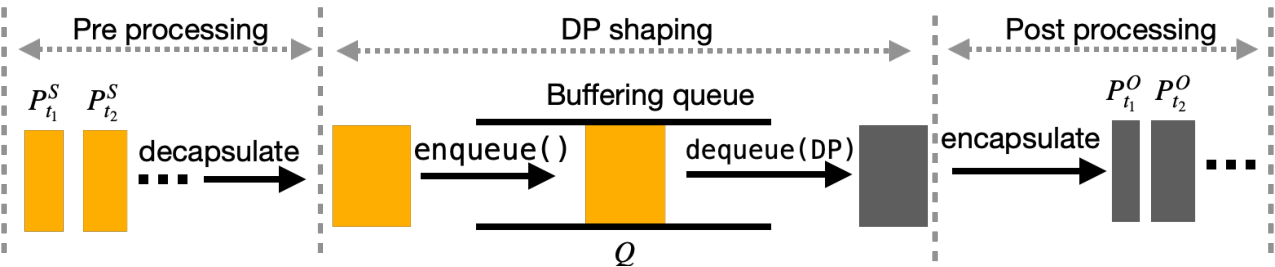
\includegraphics[width=\columnwidth]{figures/DPshaping_concept_vertical.pdf}
  %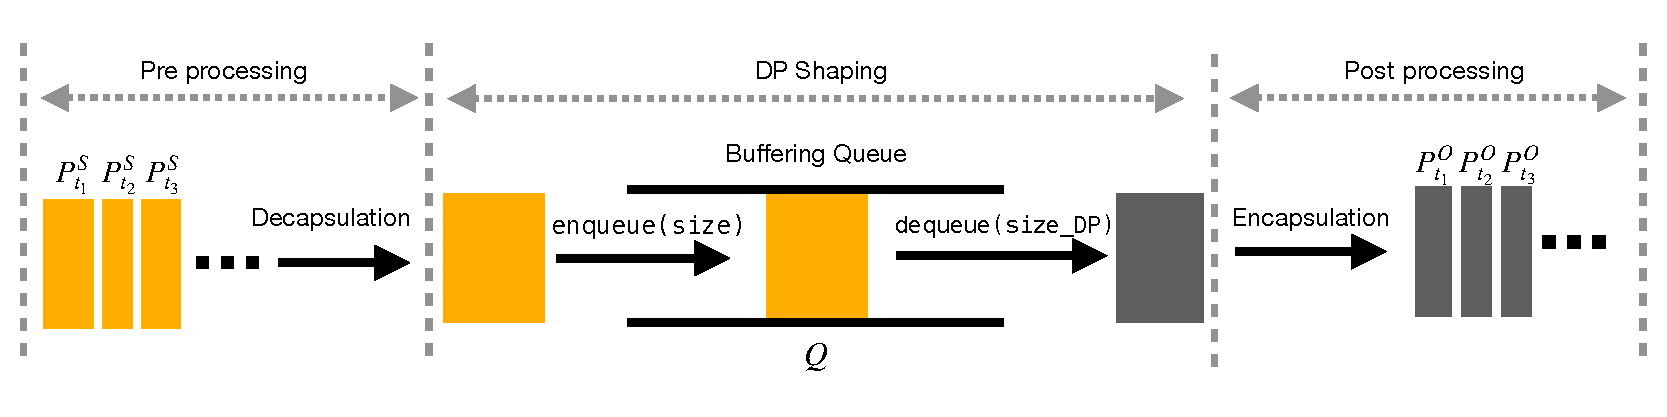
\includegraphics[width=\columnwidth]{figures/DPshaping_concept_horizontal.pdf}
  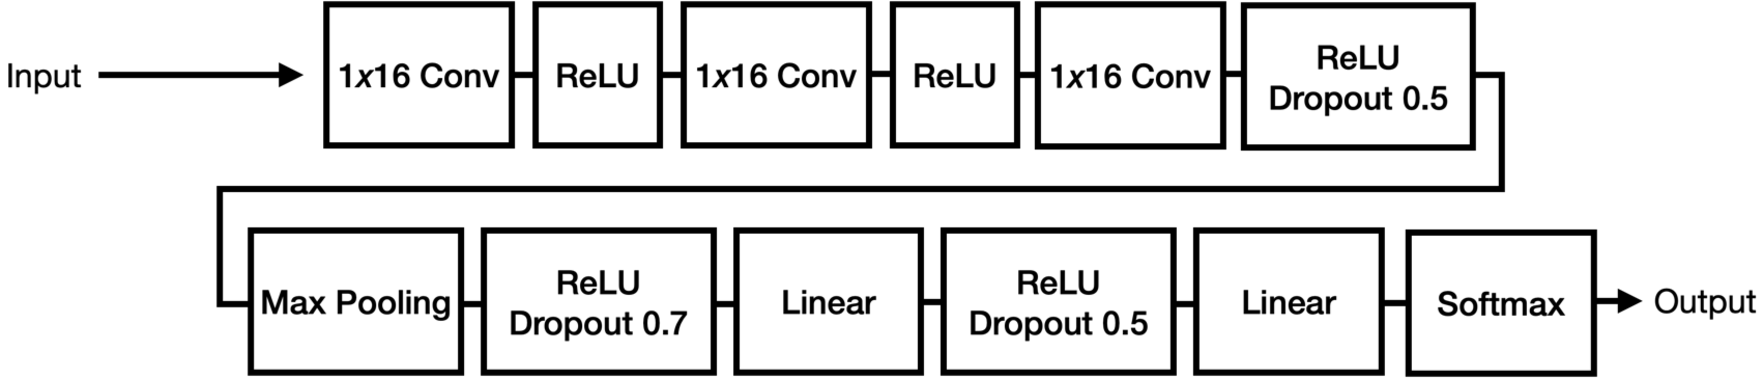
\includegraphics[width=\columnwidth]{figures/BandB_arch.pdf}
  \caption{Beauty and The Burst CNN model architecture.}
  \label{fig:bandb-arch}
\end{figure}
\subsection{TCN-based Video identification}
Beauty and the Burst~\cite{schuster2017beautyburst} uses a CNN-based architecture to for video identification. 
Convolutional neural networks have been shown to be effective in sequence modeling for decades~\cite{hinton1990connectionist}.
However, there are two problems with using a convolutional neural network as a sequence modeler.
First, convolutional layers applied to a sequence are not inherently causal, meaning that they look into future samples of a sequence to decide the output for the current sample.
Secondly, in contrast to recurrent neural networks(RNNs)~\cite{elman1990finding}, convolutional neural networks lack a deep effective history size of past samples in the sequence (i.e. their effective history is bounded to the number of samples that kernel can cover from the past).
To address these problems, Bai\etalc{bai2018empirical} proposed a new architecture called Temporal Convolutional Network (TCN).
The TCN utilizes a one-dimensional fully-convolutional network~\cite{long2015fully} equipped with causal dilated convolutions~\cite{oord2016wavenet}, allowing it to examine deep into the past to produce an output for the sequence at any given moment.
They added a generic residual block from input to output.
The architecture is shown in the \Cref{fig:tcn-arch}.
We evaluate the effectiveness of TCN model for network side-channel attacks in {\addref}




\begin{figure}[t]
  \centering
  %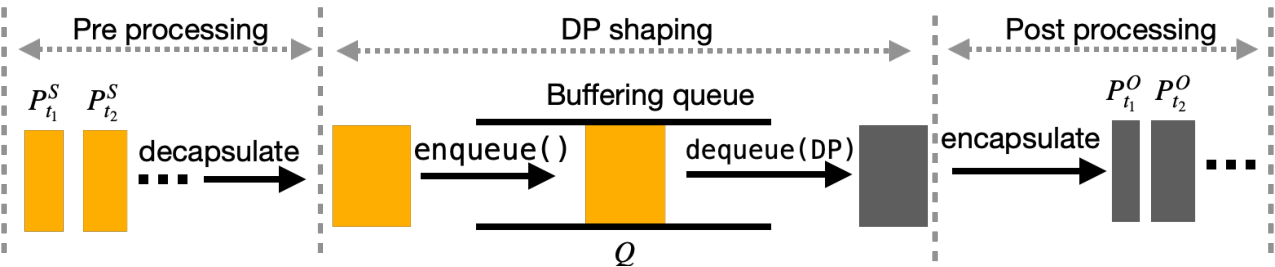
\includegraphics[width=\columnwidth]{figures/DPshaping_concept_vertical.pdf}
  %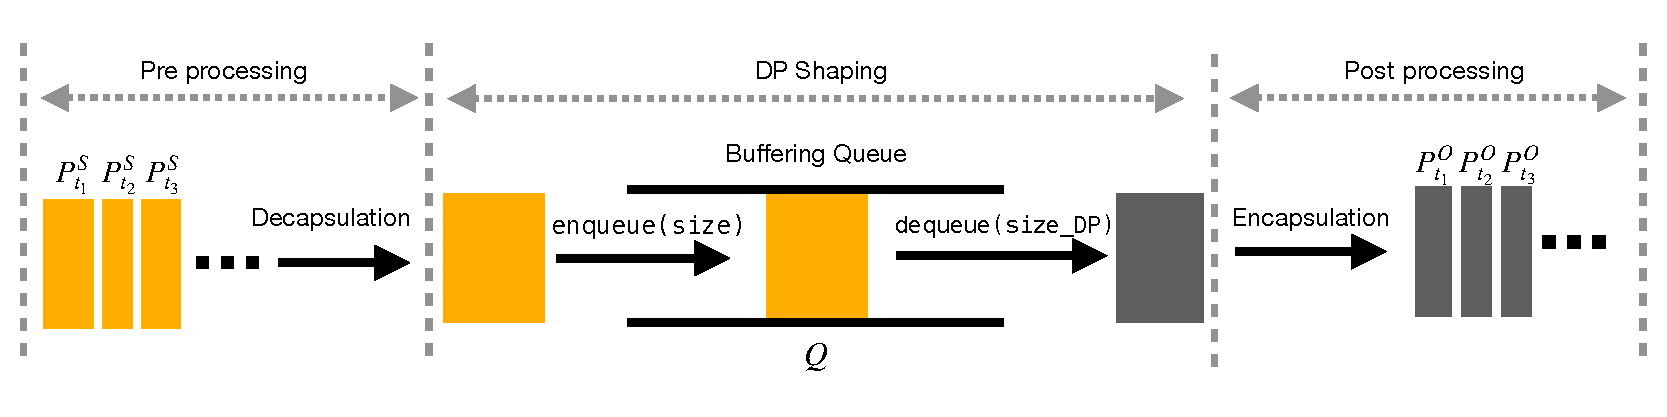
\includegraphics[width=\columnwidth]{figures/DPshaping_concept_horizontal.pdf}
  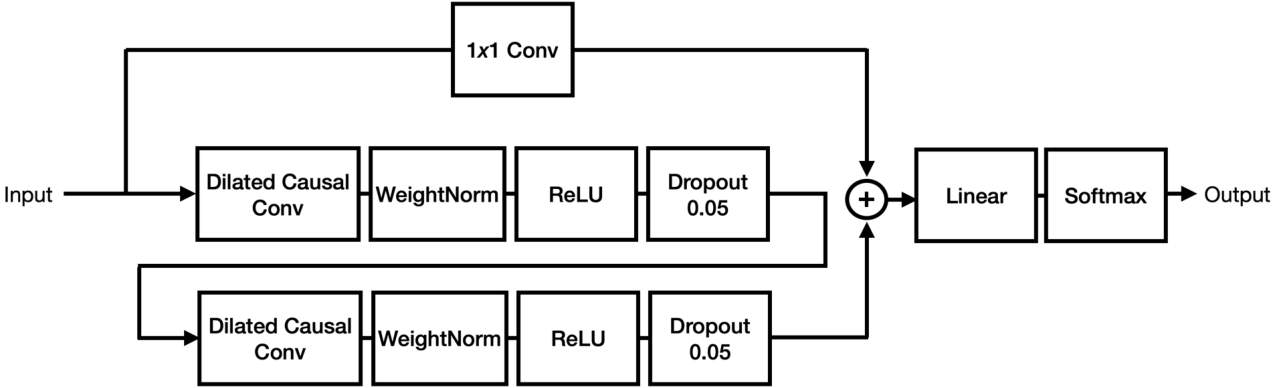
\includegraphics[width=\columnwidth]{figures/TCN_arch.pdf}
  \caption{TCN model architecture.}
  \label{fig:tcn-arch}
\end{figure}